\section{Nuclear Transparency}

The nuclear transparency was extracted as the ratio of the experimental yield
to the simulated PWIA yield from \textit{SIMC} over the phase space volume $V$
defined by the limits
$E_m<\SI{80}{\mega\electronvolt}$ and
$\norm{\vec{p}_m}<\SI{300}{\mega\electronvolt}$ for ${}^{12}C(e,e'p)$
and
$E_m<\SI{100}{\mega\electronvolt}$ and
$\norm{\vec{p}_m}<\SI{100}{\mega\electronvolt}$ for $H(e,e'p)$.
\begin{equation}
    T(Q^2) = \frac{\int_{V} d^{3} p_{m} d E_{m} Y_{exp }(E_{m}, \vec{p}_{m})}
                  {\int_{V} d^{3} p_{m} d E_{m} Y_{PWIA}(E_{m}, \vec{p}_{m})}
\end{equation}

The nuclear transparency measured as a function of $Q^2$ for $H(e,e'p)$ is
shown in Fig~\ref{fig:lh2_transparency_results}.
This elastic scattering process has no final state interactions and should be
accurately modeled by the PWIA as implemented in \textit{SIMC}.
The ratio $T$ should thus be equal to one for each point, and these
measurements are consistent with $T=1$ well within the statistical and
systematic uncertainty.
This indicates that the Monte Carlo simulation in \textit{SIMC} accurately
models the scattering process and that both the spectrometers and
\textit{hcana} are accurately reconstructing physics quantities.

% TODO: replace this with a pdf
\begin{figure}[!h]
    \centering
    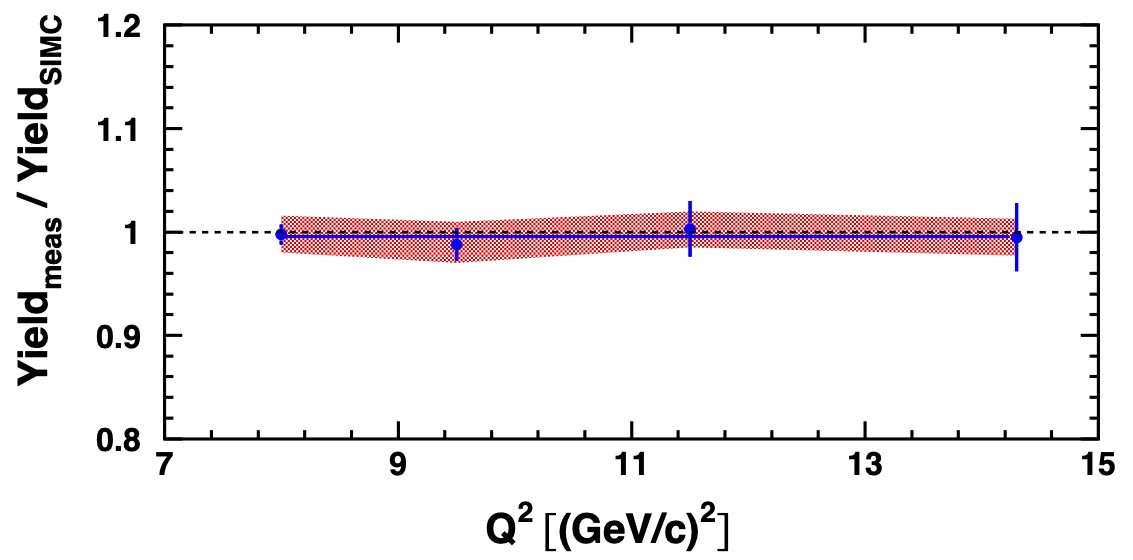
\includegraphics[width=0.8\textwidth]{chap5/lh2_results.png}
    \caption{
            Nuclear transparency for ${}^{1}H(e,e'p)$ as a function of
            momentum transfer.
            The error bars represent statistical uncertainty and the
            shaded band represents the 4.0\% systematic uncertainty.
            }
    \label{fig:lh2_transparency_results}
\end{figure}

The nuclear transparency measured as a function of $Q^2$ for ${}^{12}C(e,e'p)$
is shown in Fig~\ref{fig:lh2_transparency_results} along with previous
measurements.
Our measurements from 8--\SI{14.2}{\giga\electronvolt\squared} are consistent
with conventional multiple scattering calculations~\cite{Pandharipande_1992}
and do not support the onset of color transparency.

\begin{figure}[!h]
    \centering
    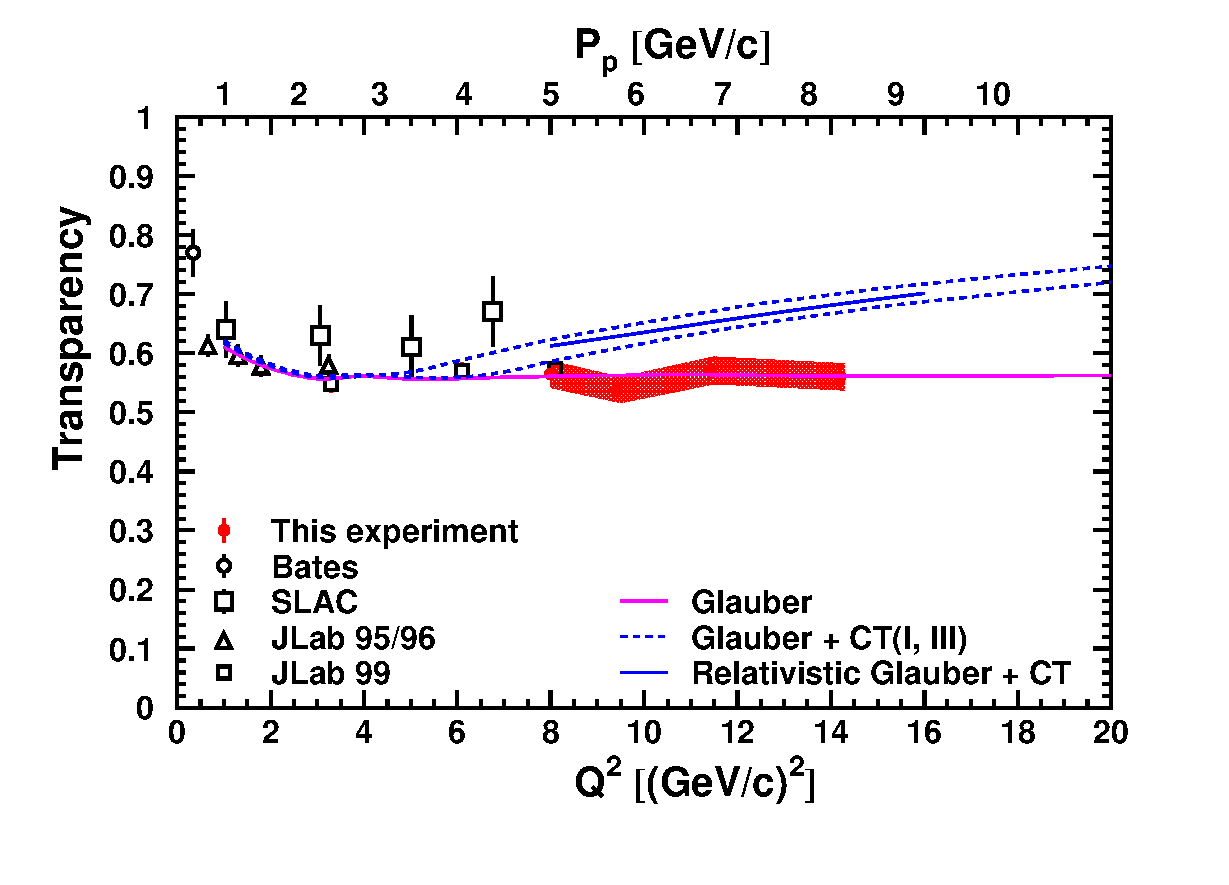
\includegraphics[width=0.8\textwidth]{chap5/c12_results.pdf}
    \caption{
            Nuclear transparency for ${}^{12}C(e,e'p)$ as a function of
            momentum transfer.
            The results of this experiment, E12-06-107, are shown in red along
            with previous measurements in open shapes.
            The error bars represent statistical uncertainty and the
            shaded band represents the 4.0\% systematic uncertainty.
            The magenta line is the prediction of a Glauber
            model that does not include CT~\cite{Pandharipande_1992}.
            The dashed lines represent predictions, for two choices of
            parameters, of a model including CT~\cite{Frankfurt_1995_PRC}.
            The solid line represents the prediction of a relativistic Glauber
            model that includes CT~\cite{Cosyn_2006}.
            }
    \label{fig:c12_transparency_results}
\end{figure}

\subsection{Systematic Uncertainty}

Table~\ref{tab:systematic_uncertainty} lists the major sources of systematic
uncertainty in our measurements of nuclear transparency.


The systematic uncertainty due to spectrometer acceptance was estimated by
taking the average of the bin-wise difference between the normalized missing
momentum spectra for data and simulation.


The uncertainty due to event selection was estimated by varying the limits of
the cuts listed in Tables~\ref{tab:lh2_cuts} and~\ref{tab:c12_cuts}
by $\pm10\%$ one at a time
and calculating the corresponding percentage change in measured transparency.
The quadrature sum of these variations was used as the systematic uncertainty.


Tracking efficiency.


Radiative corrections.


The uncertainty due to livetime and the detector efficiencies was determined
from a set of luminosity scans taken with the ${}^{12}C$ target.
The charge-normalized yield from these scans for each spectrometer was found to
be independent of the beam current within statistical uncertainties,
The average variation in the normalized yield vs beam current was recorded as the
systematic uncertainty (0.5\%).


The normalization uncertainty due to the free $ep$ cross section used in
\textit{SIMC} is 1.8\%~\cite{Bosted_1995}.
The uncertainty due to target thickness is taken from the JLab target group's
measurements. %TODO: find this citation again
The uncertainty in measured charge was estimated to be $1\%$ by varying the
minimum beam current cut used by \textit{hcana} to calculate each run's average
current.
Proton absorption.

% The total model-dependent uncertainty is 3.9\% when the uncertainty in the
% spectral function (2.8\%) and the corrections due to nucleon-nucleon
% correlations (2.7\%) are added in quadrature.

% The uncertainty in the spectral function includes the effects of the off-shell
% $\sigma_{ep}$ of 2\%, the electric and magnetic form factors of the proton
% (2\%) as previously determined\,\cite{ONeill_1995}.

\begin{table}[htb!]
    \caption{
        Systematic uncertainties in our measurements of nuclear
        transparency.
        $Q^2$-dependent uncertainties are averaged over all kinematic settings.
        The total uncertainty is the quadrature sum of the individual
        contributions.
    }
    \label{tab:systematic_uncertainty}
    \centering
    \begin{tabular}{lc}
        \hline
        \hline
        Source                            & $Q^2$-dependent uncertainty (\%) \\
        \hline
        Spectrometer acceptance           & 2.6                              \\
        Event selection                   & 1.4                              \\
        Tracking efficiency               & 0.5                              \\
        Radiative corrections             & 1.0                              \\
        Live time \& detector efficiency  & 0.5                              \\
        \hline
        \hline
        Source                            & Normalization uncertainty (\%)   \\
        \hline
        Free $ep$ cross section           & 1.8                              \\
        Target thickness                  & 0.5                              \\
        Beam charge                       & 1.0                              \\
        Proton absorption                 & 1.2                              \\
        \hline
        \hline
        Total                             & 4.0                              \\
    \end{tabular}
\end{table}
